%%%%%%%%%%%%%%%%%%%%%%%%%%%%%%%%%%%%%%%%%%%%%%%%%%%%%%%%%%%%%%%
%
% Welcome to Overleaf --- just edit your LaTeX on the left,
% and we'll compile it for you on the right. If you open the
% 'Share' menu, you can invite other users to edit at the same
% time. See www.overleaf.com/learn for more info. Enjoy!
%
%%%%%%%%%%%%%%%%%%%%%%%%%%%%%%%%%%%%%%%%%%%%%%%%%%%%%%%%%%%%%%%


% Inbuilt themes in beamer
\documentclass{beamer}

% Theme choice:
\usetheme{CambridgeUS}

% Packages
\usepackage{graphicx}
\graphicspath{{images/}}
\usepackage{gensymb}
\usepackage{amssymb}
\usepackage[cmex10]{amsmath}
\usepackage{amsthm}
\usepackage[export]{adjustbox}
\usepackage{bm}
\usepackage{longtable}
\usepackage{enumitem}
\usepackage{mathtools}
 \usepackage{tikz}
\usepackage[breaklinks=true]{hyperref}
\usepackage{listings}
\usepackage{color}                                            %%
\usepackage{array}                                            %%
\usepackage{longtable}                                        %%
\usepackage{calc}                                             %%
\usepackage{multirow}                                         %%
\usepackage{hhline}                                           %%
\usepackage{ifthen}                                           %%
\usepackage{lscape}     
\usepackage{multicol}
\usepackage{enumerate}
\DeclareMathOperator*{\Res}{Res}
\renewcommand\thesection{\arabic{section}}
\renewcommand\thesubsection{\thesection.\arabic{subsection}}
\renewcommand\thesubsubsection{\thesubsection.\arabic{subsubsection}}
\renewcommand\thesectiondis{\arabic{section}}
\renewcommand\thesubsectiondis{\thesectiondis.\arabic{subsection}}
\renewcommand\thesubsubsectiondis{\thesubsectiondis.\arabic{subsubsection}}
\hyphenation{op-tical net-works semi-conduc-tor}
\def\inputGnumericTable{}                                 %%
\lstset{
frame=single, 
breaklines=true,
columns=fullflexible
}

\newcommand{\BEQA}{\begin{eqnarray}}
\newcommand{\EEQA}{\end{eqnarray}}
\newcommand{\define}{\stackrel{\triangle}{=}}
\newcommand*\circled[1]{\tikz[baseline=(char.base)]{
    \node[shape=circle,draw,inner sep=2pt] (char) {#1};}}
%\bibliographystyle{IEEEtran}
\providecommand{\mbf}{\mathbf}
\providecommand{\pr}[1]{\ensuremath{\Pr\left(#1\right)}}
\providecommand{\qfunc}[1]{\ensuremath{Q\left(#1\right)}}
\providecommand{\sbrak}[1]{\ensuremath{{}\left[#1\right]}}
\providecommand{\lsbrak}[1]{\ensuremath{{}\left[#1\right.}}
\providecommand{\rsbrak}[1]{\ensuremath{{}\left.#1\right]}}
\providecommand{\brak}[1]{\ensuremath{\left(#1\right)}}
\providecommand{\lbrak}[1]{\ensuremath{\left(#1\right.}}
\providecommand{\rbrak}[1]{\ensuremath{\left.#1\right)}}
\providecommand{\cbrak}[1]{\ensuremath{\left\{#1\right\}}}
\providecommand{\lcbrak}[1]{\ensuremath{\left\{#1\right.}}
\providecommand{\rcbrak}[1]{\ensuremath{\left.#1\right\}}}
\theoremstyle{remark}
\newtheorem{rem}{Remark}
\newcommand{\sgn}{\mathop{\mathrm{sgn}}}
%\providecommand{\abs}[1]{\left\vert#1\right\vert}
%\providecommand{\res}[1]{\Res\displaylimits_{#1}} 
%\providecommand{\norm}[1]{\left\lVert#1\right\rVert}
%\providecommand{\norm}[1]{\lVert#1\rVert}
%\providecommand{\mtx}[1]{\mathbf{#1}}
%\providecommand{\mean}[1]{E\left[ #1 \right]}
\providecommand{\fourier}{\overset{\mathcal{F}}{ \rightleftharpoons}}
%\providecommand{\hilbert}{\overset{\mathcal{H}}{ \rightleftharpoons}}
\providecommand{\system}{\overset{\mathcal{H}}{ \longleftrightarrow}}
	%\newcommand{\solution}[2]{\textbf{Solution:}{#1}}
\newcommand{\solution}{\noindent \textbf{Solution: }}
\newcommand{\cosec}{\,\text{cosec}\,}
\providecommand{\dec}[2]{\ensuremath{\overset{#1}{\underset{#2}{\gtrless}}}}
\newcommand{\myvec}[1]{\ensuremath{\begin{pmatrix}#1\end{pmatrix}}}
\newcommand{\mydet}[1]{\ensuremath{\begin{vmatrix}#1\end{vmatrix}}}
\newcommand*{\permcomb}[4][0mu]{{{}^{#3}\mkern#1#2_{#4}}}
\newcommand*{\perm}[1][-3mu]{\permcomb[#1]{P}}
\newcommand*{\comb}[1][-1mu]{\permcomb[#1]{C}}
\numberwithin{equation}{subsection}
\makeatletter
\@addtoreset{figure}{problem}
\makeatother
\let\StandardTheFigure\thefigure
\let\vec\mathbf
\renewcommand{\thefigure}{\theproblem}
\def\putbox#1#2#3{\makebox[0in][l]{\makebox[#1][l]{}\raisebox{\baselineskip}[0in][0in]{\raisebox{#2}[0in][0in]{#3}}}}
     \def\rightbox#1{\makebox[0in][r]{#1}}
     \def\centbox#1{\makebox[0in]{#1}}
     \def\topbox#1{\raisebox{-\baselineskip}[0in][0in]{#1}}
     \def\midbox#1{\raisebox{-0.5\baselineskip}[0in][0in]{#1}}
\vspace{3cm}


% Title page details: 
\title{Assignment 9} 
\author{Hema Sri Cheekatla, CS21BTECH11013}
\date{\today}
\logo{\large \LaTeX{}}


\begin{document}
% Title page frame
\begin{frame}
    \titlepage 
\end{frame}

% Remove logo from the next slides
\logo{}


% Outline frame
\begin{frame}{Outline}
    \tableofcontents
\end{frame}

% Question frame
\begin{frame}{Question}
    \section{Question:}
    x, y are independent uniformly distributed random variables in (0, 1). Let
    \begin{align}
        w &= max(x,y) \\
        z &= min(x, y) 
    \end{align}
    Find the p.d.f of
    \begin{itemize}
        \item[(a)] $r=w-z$
        \item[(b)] $s = w+z$ 
    \end{itemize}
\end{frame}

% Solution Frames
\begin{frame}{Solution(a)}
    \section{Solution:}
    \begin{align}
        R &= W-Z \\
        &= max(X, Y) - min(X, Y) \\
        &= \begin{cases} X-Y &, X \geq Y \\
        Y - X &, X < Y\end{cases} \\
        \text{Hence, } F_R(r) &= \pr{R \leq r} \\
        &= \pr{X-Y \leq r, X \geq Y} + \pr{Y -X \leq r, X < Y}
    \end{align}
\end{frame}

\begin{frame}{Solution(a)}
    The corresponding regions are shaded as below, where we are given that x,y are in (0,1)
    \begin{figure}[h]
        \centering
        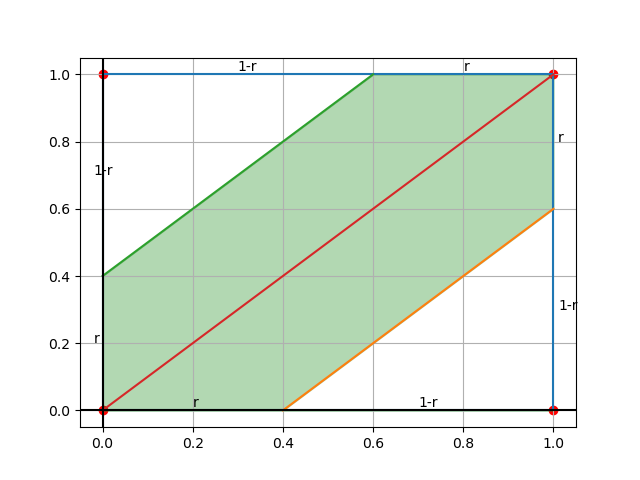
\includegraphics[width = 0.5\textwidth]{plot1.png}
        \caption{The possible region}
        \label{fig:my_label}
    \end{figure}
\end{frame}

\begin{frame}{Solution(a)}
    From the plot, The area is given by,
    \begin{align}
        F_R(r) &= 1 - 2\frac{(1-r)^2}{2}, 0 \leq r \leq 1 \\
        &= 1 - (1-r)^2
    \end{align}
    Hence the p.d.f is written as follows,
    \begin{align}
        p_R(r) &= \frac{d}{dr} F_R(r) \\
        p_R(r) &= \frac{d}{dr} (1 - (1-r)^2) \\
        p_R(r) &= \begin{cases} 2(1-r) &, 0 \leq r \leq 1 \\
       0 &, otherwise\end{cases}
    \end{align}
\end{frame}

\begin{frame}{Solution(b)}
    \begin{align}
        S &= W+Z \\
        &= max(X, Y) + min(X, Y) \\
        &= \begin{cases} X+Y &, X \geq Y \\
        Y + X &, X < Y\end{cases} \\
        S &= X+Y, X,Y \in (0, 1) \\
        \text{Hence, } F_S(s) &= \pr{S \leq s} \\
        &= \pr{X+Y \leq s}, 0 < s < 2 \\
    \end{align}
\end{frame}

\begin{frame}{Solution(b)}
    For $0 < s < 1$, the range is given below,
    \begin{figure}
        \centering
        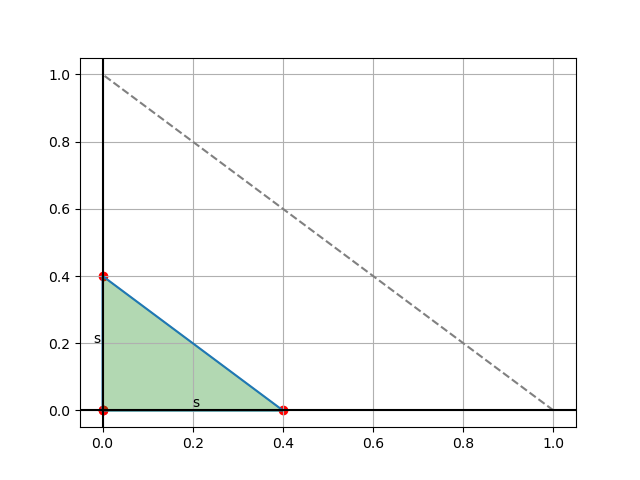
\includegraphics[width=0.5\textwidth]{plot2.png}
        \caption{for $0<s<1$}
        \label{fig:my_label}
    \end{figure}
    \begin{align}
        F_S(s) &= \frac{1}{2} s^2, 0<s<1
    \end{align}
\end{frame}

\begin{frame}{Solution(b)}
    for $1<s<2$, the possible range is given as follows,
    \begin{figure}
        \centering
        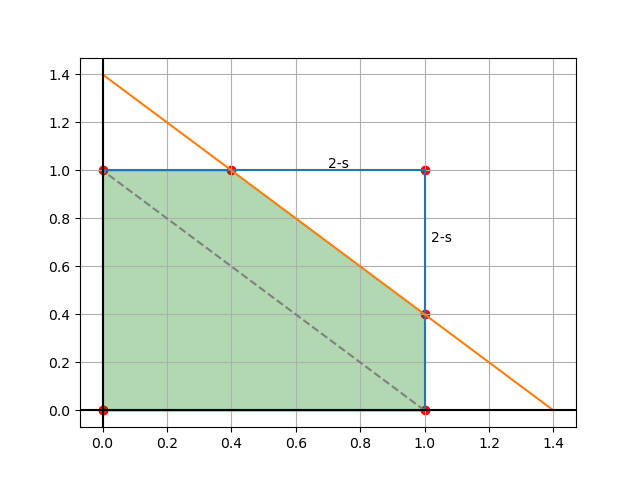
\includegraphics[width=0.5\textwidth]{plot3.png}
        \caption{For $1<s<2$}
        \label{fig:my_label}
    \end{figure}
    \begin{align}
        \implies F_s(s) &= 1 - \frac{1}{2}(2-s)^2, 1<s<2
    \end{align}
\end{frame}

\begin{frame}{Solution(b)}
    \begin{align}
        F_S(s) &= \begin{cases} \frac{s^2}{2} &, 0<s<1 \\
        1-\frac{(2-s)^2}{2} &, 1<s<2 \end{cases}
    \end{align}
    Hence the p.d.f of S is given as follows,
    \begin{align}
        p_S(s) &= \frac{d}{ds} F_S(s) \\
        &= \begin{cases} \frac{d}{ds}(\frac{s^2}{2}) &, 0<s<1 \\
        \frac{d}{ds}(1-\frac{(2-s)^2}{2}) &, 1<s<2 \end{cases} \\
        &= \begin{cases} s &, 0<s<1 \\
        2-s, &1<s<2\\
        0 &, otherwise\end{cases}
    \end{align}
\end{frame}

\begin{frame}{Solution}
    pdf of R,
    \begin{align}
        p_R(r) &= \begin{cases} 2(1-r) &, 0 \leq r \leq 1 \\
       0 &, otherwise\end{cases}
    \end{align}
    pdf of S, 
    \begin{align}
        p_S(s)&= \begin{cases} s &, 0<s<1 \\
        2-s, &1<s<2\\
        0 &, otherwise\end{cases}
    \end{align}
\end{frame}
\end{document}
